\textsf{Cassis} est un simulateur de caches sur architecture multi-c\oe ur développé dans le cadre d'un PFA -- Projet au Fil de l'Année -- à l'\textsc{Enseirb-Matmeca}, sur une idée proposée par Denis BARTHOU pour le compte de l'\textsf{INRIA}. L'\textsf{INRIA} est un institut publique de recherche français en informatique et automatismes ; et bien que ce projet soit réalisé dans un cadre scolaire, l'objectif est de le rendre utilisable par les équipes de recherche des thématiques associées aux caches et au parallèlisme.

\section{Cadre du simulateur}

\paragraph{}
Un simulateur est un programme qui va reproduire le fonctionnement d'un système afin de pouvoir en étudier certaine caractéristiques de manière moins contraignante que sur le système réel. Dans le cas du programme \textsc{Cassis}, c'est l'utilisation des caches par un programme donné qui est simulée.

\subsection{Origine du projet}

\paragraph{}
La mémoire est un facteur de ralentissement des programmes très important de nos jours. Une mauvaise gestion de la mémoire peut être désastreuse au niveau des performances, et pourtant, il n'existe pas de moyen efficace et précis de connaître l'utilisation de la mémoire au niveau des caches. Le but de \textsf{Cassis} est donc d'étudier l'utilisation précise des caches par un programme, afin d'aider l'utilisateur à tester les performances du programmes, ainsi que les analyser pour les améliorer.

\paragraph{}
Le besoin d'un tel simulateur est avant tout dû au manque d'informations des caches. Deux phénomènes se produisent du côté des constructeurs de processeurs. D'une part ils doivent les optimiser afin d'être concurrents, et il devient alors difficile pour eux de rajouter des fonctionnalités dédiées aux développeurs afin d'améliorer leur code, par exemple des compteurs exacts du nombre de \emph{hits}. D'autre part il n'est pas dans leur intérêt de révéler le fonctionnement de leurs produits, pour des raisons économiques évidentes. Par exemple, le \emph{prefetching} permet de charger des lignes de caches en avance en fonction des accès mémoires courants du programme et cette fonctionnalité n'est pas implémentée dans le simulateur car son fonctionnement n'est pas totalement divulgué.

\paragraph{}
L'intérêt d'un tel simulateur est donc de pouvoir tester des programmes en produisant certaines statistiques, mais aussi de pouvoir tester l'exécution sur des architectures qui n'existent pas afin de connaître la pertinence d'une nouvelle politique de cohérence par exemple.

\subsection{Données simulées : analyses possibles des résultats}

Différentes statistiques sont relevées par le simulateur, les principales sont les \emph{misses}, les \emph{hits} et les \emph{write-backs}. Il est aussi possible de connaître le nombre de messages envoyés sur le bus par un cache afin d'effectuer la cohérence, ainsi que le nombre de données qui ont été invalidées à cause de la cohérence ou à cause de l'inclusivité, et enfin comment la donnée a été atteinte (qui l'a transmis au cache s'il ne l'avait pas : son parent, ou un cache de même niveau). Une sortie classique serait donc :

\begin{lstlisting}
L3  basics   (misses:   6, hits:   0, writes_back:   0)
L2  basics   (misses:   6, hits:   0, writes_back:   0)
L1  basics   (misses:   4, hits:  44, writes_back:   1)
L1  basics   (misses:   6, hits:  42, writes_back:   2)
L2  basics   (misses:   0, hits:   0, writes_back:   0)
L1  basics   (misses:   0, hits:   0, writes_back:   0)
L1  basics   (misses:   0, hits:   0, writes_back:   0)
\end{lstlisting}

\paragraph{}
Ces statistiques ont été choisie afin que l'utilisateur puisse constater certains problèmes particuliers. En effet un nombre trop élevé de \emph{write-backs} et/ou de \emph{coherence evinctions} révèlent que les c\oe urs modifient les mêmes données et que le parallélisme n'est donc pas bien réalisé. Mais les statistiques ne sont pas les seuls paramètres d'analyse, la sélection des données à analyser à aussi un rôle important. Le simulateur permet de suivre les statistiques d'une ou plusieurs instructions données, et ainsi de déterminer quelles instructions causent des ralentissements à l'exécution, i.e. un trop grand nombre de \emph{misses}.

\subsection{Outils à disposition de l'utilisateur}

Le simulateur s'appuie sur des outils préexistants, pour la génération des traces et de l'architecture. Les outils listés ci-dessous sont ceux utilisés par l'équipe de projet. Si d'autres outils offrent des fonctionnalités similaires, ils peuvent être utilisés en remplacement tant que les fichiers d'entrée du programme sont dans le bon format.

\paragraph{HWLOC} est un logiciel qui permet de récupérer l'architecture des caches d'une machine. Il permet de générer un fichier xml que nous enrichissons. La paramétrisation de l'architecture des caches ne prend pas en compte les caches d'instructions, mais seulement les caches de données. L'utilisation de ce fichier est détaillé dans la section \ref{param_xml}.

\paragraph{MAQAO} (Modular Assembly Quality Analyzer and Optimizer) est un outil d'analyse et d'optimisation de programmes. Une seule fonctionnalité de \textsf{MAQAO} est utilisée, celle qui permet d'instrumenter un programme binaire afin de récupérer les opérations faites lors de l'exécution. Le paramétrage de \textsf{MAQAO} est effectué grâce à un fichier lua pour générer des traces de la forme voulue.

\paragraph{}
L'utilisateur peut aussi vouloir comparer les résultats de la simulation. Bien qu'il n'existe par actuellement de tel simulateur pour faire la comparaison, il existe des compteurs hardware --par exemple \textsf{PAPI} -- qui permettent de connaître certaines statistiques sur les caches. Ces statistiques sont celles desquelles il faudrait le plus se rapprocher, bien qu'elles ne soient pas non plus exactes.


\section{Déroulement de la simulation}

\paragraph{}
La simulation consiste à rejouer un certain nombre d'instructions, et de comptabiliser certaines métriques à destination de l'utilisateur. Comme il s'agit d'une simulation, tout ne se passe pas exactement comme dans le cas réel. Il est donc nécessaire d'expliciter les similitudes comme les différences afin que l'utilisateur ne soit pas surpris à la fois par les résultats, et à la fois par les méthodes de calculs si son objectif est de modifier le code.

\subsection{Traitement d'une instruction : load/store}

\paragraph{}
La simulation, même d'un programme parallèle, est une séquence d'instructions effecutant des modifications (lecture ou écriture) sur les caches. Les deux premières possibilités pour une instruction sont soit une lecture de donnée, soit une écriture. Une fois cela déterminé, il faut savoir où se trouve la donnée, elle peut déjà être dans le cache, ou dans un de ses voisins, ou dans un de ses parents. La donnée est alors rappatriée en prévenant les autres caches de l'action en cours. 

\paragraph{}
Tous les caches concernés appliquent alors la politique de cohérence : une action a été faite sur la donnée, elle a été lue ou modifiée, par un autre cache ou par soi-même. L'automate change alors l'état de la ligne suivant la nature de la transition. Il faut aussi penser à gérer le cas ou le cache est plein : le rappatriement d'une donnée donne alors lieu à la suppression d'une autre, il faut aussi propager cette information, et veiller à la cohérence de la donnée dans le reste de l'architecture.

\paragraph{}
L'ordre des tests est le suivant : 
\begin{enumerate}
  \item{il s'agit d'un \emph{load} ou d'un \emph{store}}
  \item{la donnée est présente dans le cache ou non (récursif)
    \begin{enumerate}
      \item{si non, l'ajouter et faire :}
      \item{appel de la procédure de suppression en cas de cache plein}
      \item{prévenir le cache supérieur que la donnée est accédée}
      \item{revenir au point 2}
  \end{enumerate}}
  \item{modifier les statistiques d'utilisation de la ligne}
  \item{dans le cas d'un \emph{store}, propager l'action de modification dans tous les caches de niveaux supérieurs}
\end{enumerate}

\paragraph{}
Dans le code du simulateur, le traitement d'une instruction est ainsi différent s'il s'agit d'un \emph{load} ou d'un \emph{store}. En effet les deux versions se distinguent par la dernière étape dans le cas d'un \emph{store}, qui nécessite de prévenir tous les caches parents. En effet si la donnée est simplement lue, il n'y a pas lieu de prévenir les caches parents, ni d'augmenter les statistiques de la ligne dans ces caches.

\subsection{Rapatriement prédictif d'une ligne}

\paragraph{}
Les étapes précédentes de l'algorithme montrent que la ligne est ajoutée avant même que les caches de niveau supérieur aient confirmé qu'ils l'ont ou non. Contrairement au cas réel, nous considérons donc que nous avons la donnée dans tous les cas, et nous propageons uniquement la demande aux niveaux supérieurs. Cela augement la rapidité car il n'y a pas d'aller/retour de messages entre les niveaux de caches, ceux-ci ne font \emph{a priori} que monter vers les caches supérieurs.

\paragraph{}
Cette particularité est à prendre en compte dans l'écriture des politiques de cohérences. En effet certaines politiques se basent sur la présence ou non de la même ligne dans le niveau du cache demandant la donnée, voir à ce sujet les conditions de transitions d'automates dans la partie \ref{aut}. Il faut alors être conscient que la donnée est déjà dans le niveau lorsque les voisins sont prévenus.

\paragraph{}
En résumé il faut considérer que le cache effectuant la requête de ligne l'ajoute, prévient ses voisins, puis prévient le niveau supérieur. La cohérence entre les niveaux est toujours assurée, mais celle sur le niveau-même n'est donc pas exactement la même que dans le cas réel où les voisins sont informés avant l'ajout effectif de la ligne.


\subsection{Problème d'ajout de ligne dans un cache plein}


Donner exemples montrant la nécessité de \verb:not_rm:.

\subsection{\'Etapes de validation}
\begin{frame}
  \begin{block}{Pr\'esentation}
    \begin{itemize}
      \item Tests unitaires
      \item Validation durant le programme
      \item Comparaison avec des outils existants
      \item Benchmarks
    \end{itemize}
  \end{block}
  \begin{block}{Premiers outils de v\'erification}
    \begin{itemize}
      \item Validation des politiques basiques
      \item Validation du comportement inclusif
      \item Utilisation de \textsf{PAPI}
    \end{itemize}
  \end{block}
\end{frame}

\begin{frame}{Benchmarks basiques}
\begin{figure}[H]
   \begin{minipage}[l]{.46\textwidth}
     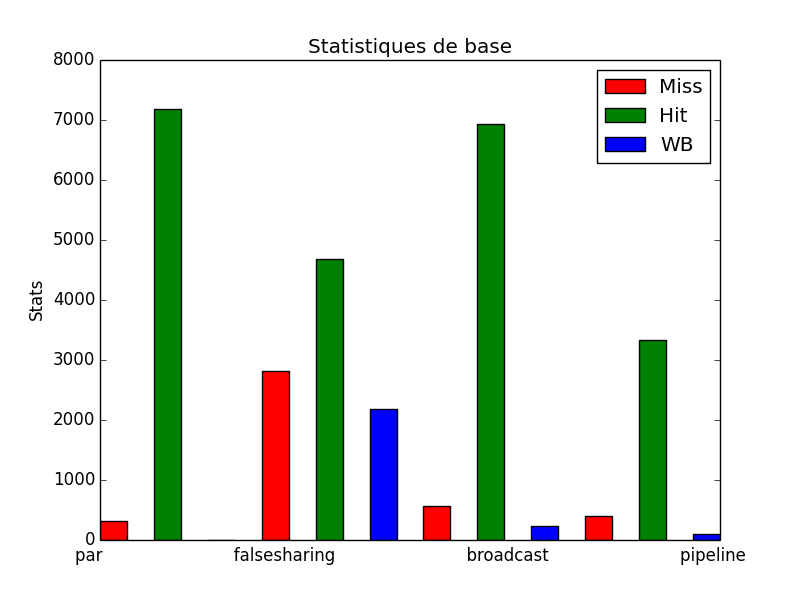
\includegraphics[scale=0.22]{images/stats_L1.png}
   \end{minipage} \hfill
   \begin{minipage}[r]{.46\textwidth}
     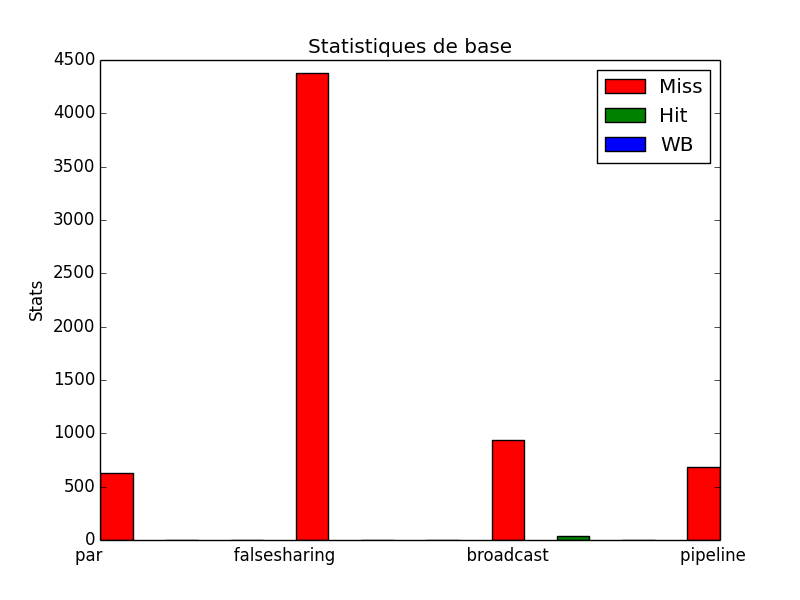
\includegraphics[scale=0.22]{images/stats_L2.png}
   \end{minipage}
\end{figure}

\begin{figure}[t!]
  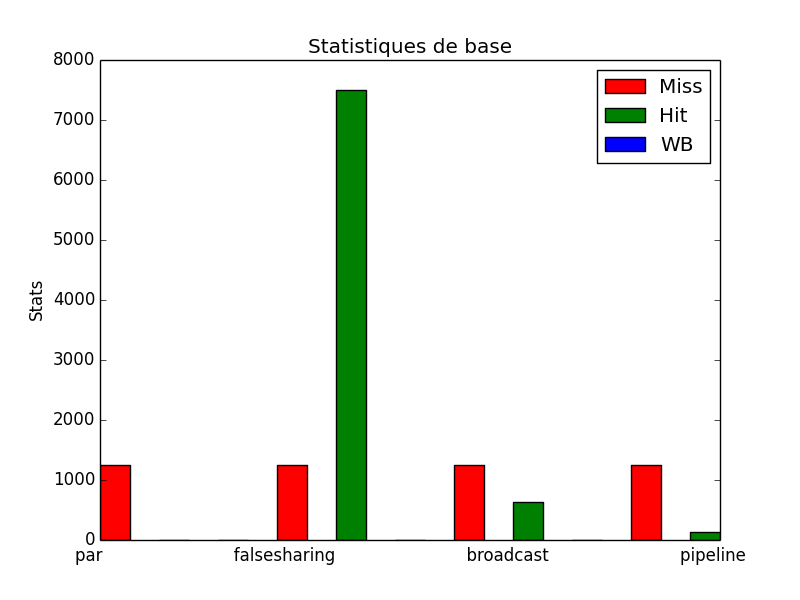
\includegraphics[scale=0.22]{images/stats_L3.png}
\end{figure}
\end{frame}

\begin{frame}{Benchmarks avanc\'es}
\begin{figure}[H]
   \begin{minipage}[l]{.46\textwidth}
     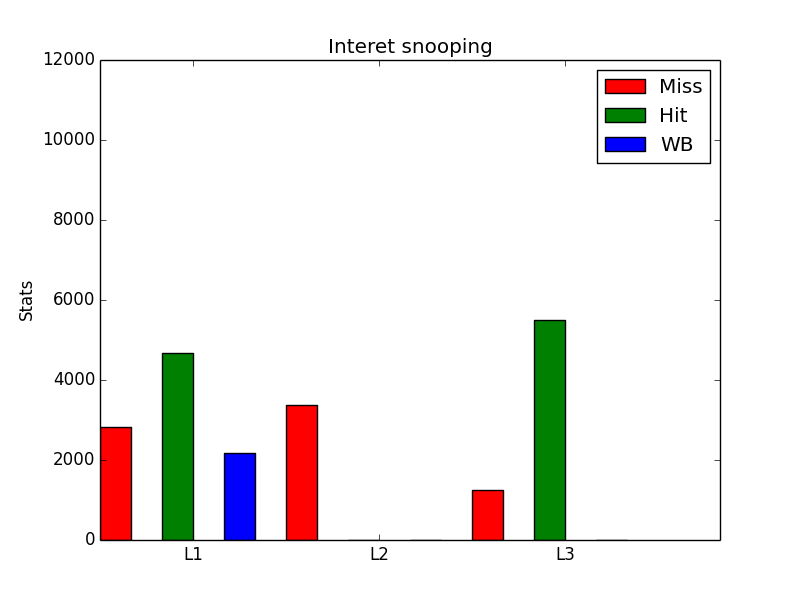
\includegraphics[scale=0.22]{images/stats_falsesharing_snooping.png}
   \end{minipage} \hfill
   \begin{minipage}[r]{.46\textwidth}
     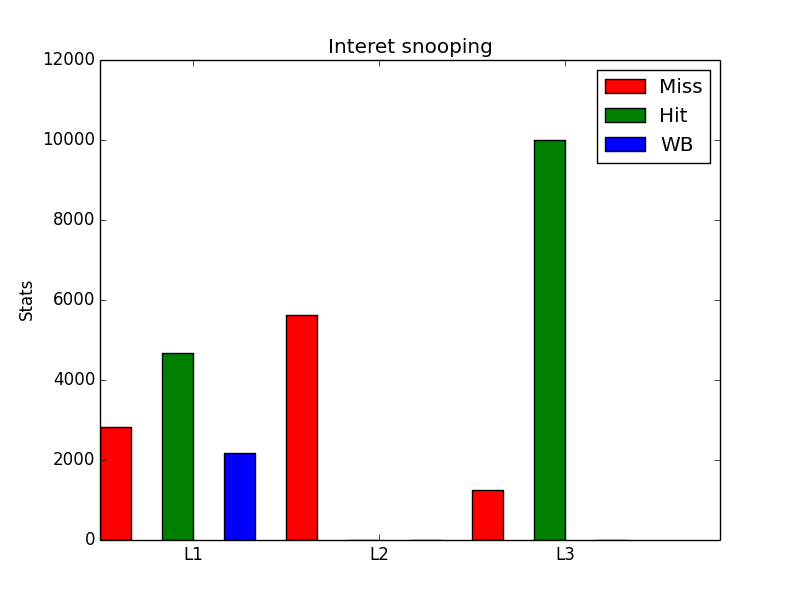
\includegraphics[scale=0.22]{images/stats_falsesharing_no_snooping.png}
   \end{minipage}
\end{figure}
  \begin{block}{Autres benchmarks}
    \begin{itemize}
      \item \emph{Directory manager}
      \item Politiques de coh\'erence MSI vs MESI
      \item Scalabilit\'e
    \end{itemize}
  \end{block}
\end{frame}

\subsection{Limites \`a  propos de la simulation des caches}
\begin{frame}
  \begin{block}{Probl\`emes li\'es aux architectures multi-c{\oe}ur}
    \begin{itemize}
      \item \textsf{prefetching}
      \item synchronisations
      \item changements de contextes 
    \end{itemize}
  \end{block}
  \begin{block}{Limites de \textsf{Cassis}}
    \begin{itemize}
      \item bande passante non mod\'elis\'ee
      \item \textsf{Directory manager} basiquement mod\'elis\'es
      \item statistiques non calibr\'ees avec des benchmarks classiques
      \item utilisation de m\'etriques non usuelles
    \end{itemize}
  \end{block}
\end{frame}


\section*{Conclusion}
\begin{frame}
  \begin{block}{Objectifs atteints}
    \begin{itemize}
      \item Cahier des charges respect\'e
      \item Param\'etrisation compl\`ete
    \end{itemize}
  \end{block}

  \begin{block}{\'Evolution possible}
    \begin{itemize}
      \item Complage avec un simulateur \textsf{on-line}?
      \item Utilisation de benchmarks pour calibrer les r\'esultats?
    \end{itemize}
  \end{block}
\end{frame}

